\section{SearchController Class Reference}
\label{classSearchController}\index{SearchController@{SearchController}}
Inheritance diagram for SearchController:\nopagebreak
\begin{figure}[H]
\begin{center}
\leavevmode
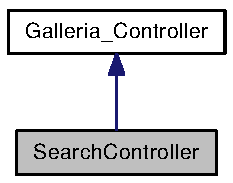
\includegraphics[width=74pt]{classSearchController__inherit__graph}
\end{center}
\end{figure}
Collaboration diagram for SearchController:\nopagebreak
\begin{figure}[H]
\begin{center}
\leavevmode
\includegraphics[width=74pt]{classSearchController__coll__graph}
\end{center}
\end{figure}
\subsection*{Public Member Functions}
\begin{CompactItemize}
\item 
{\bf indexAction} ()
\end{CompactItemize}


\subsection{Detailed Description}


Definition at line 19 of file searchcontroller.php.

\subsection{Member Function Documentation}
\index{SearchController@{SearchController}!indexAction@{indexAction}}
\index{indexAction@{indexAction}!SearchController@{SearchController}}
\subsubsection{\setlength{\rightskip}{0pt plus 5cm}SearchController.indexAction ()}\label{classSearchController_23220fa63c8d9c3ccad8c50cd6a7195e}


Index page.

Index page action. Sets up Search index page.  public 

Definition at line 28 of file searchcontroller.php.

References Galleria\_\-Controller.\_\-getModel(), and Galleria\_\-Controller.getView().

Here is the call graph for this function:\nopagebreak
\begin{figure}[H]
\begin{center}
\leavevmode
\includegraphics[width=195pt]{classSearchController_23220fa63c8d9c3ccad8c50cd6a7195e_cgraph}
\end{center}
\end{figure}


The documentation for this class was generated from the following file:\begin{CompactItemize}
\item 
/var/www/galleria/data/site/mvc/controller/{\bf searchcontroller.php}\end{CompactItemize}
